\documentclass[mathserif]{beamer}
\usepackage[ngerman]{babel}
\usepackage[latin1]{inputenc}
\usepackage{amsmath, amssymb}
\usepackage{latexsym}
%
\newcommand{\R}{\mathbb{R}}
\usetheme{Madrid}
\usecolortheme{seahorse}
%
%
\title[MNS Project 2]{MNS Project 2: Learning of Grid Cells}
\author[C. Lang, E. Sezener, C.Winklmayr]{Claus Lang, Eren Sezener and Claudia Winklmayr}
\institute{BCCN}
\date[9.2.2016]{February $9^{th}$ 2016}
%
\begin{document}
\maketitle
%
%
\begin{frame}
\frametitle{Introduction}
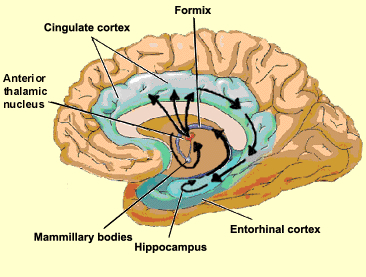
\includegraphics[width=0.7\textwidth]{mEC.jpg}\newline
%http://www.irafs.org/images/irafs_nl_eng_2_files/image007.jpg
In Hippocampus and the medial enthorhinal cortex (mEC) various types of neurones have been found that encode an animals spacial location.  
\end{frame}
% 
%
%
\begin{frame}
\frametitle{Cells encoding spacial location}
\begin{itemize}
\item \textbf{Place cells:} Located in hippocampus. Activated when the animal enters a specific region of the environment - the \textit{place field]}. \newline
%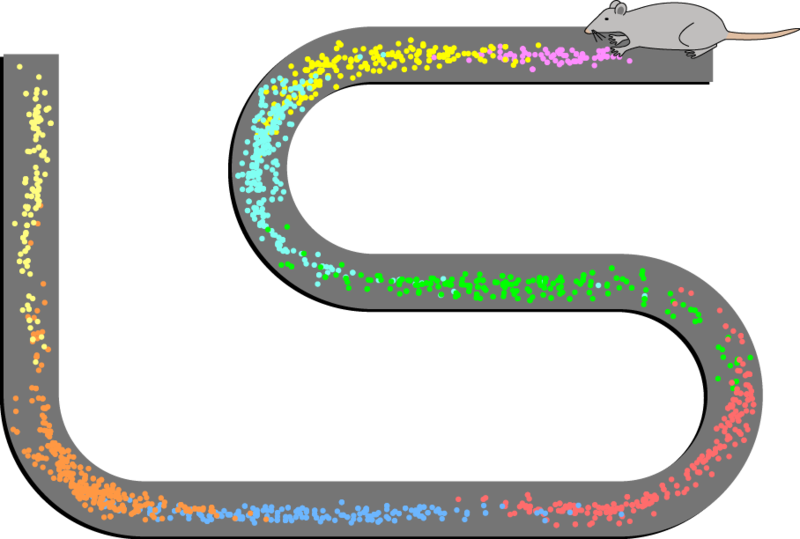
\includegraphics[width=0.33\textwidth]{Place_Cell_Spiking_Activity_Example.png}
%"Place Cell Spiking Activity Example" by Stuartlayton at English Wikipedia. Licensed under CC BY-SA 3.0 via Commons - https://commons.wikimedia.org/wiki/File:Place_Cell_Spiking_Activity_Example.png#/media/File:Place_Cell_Spiking_Activity_Example.png
\item \textbf{Grid cells:} Located in  medial enthorhinal cortex (mEC). Activated at several spacial positions. The firing map shows an equally spaced hexagonal pattern. \newline
\item \textbf{Head-direction cells}\newline
\item \textbf{Head-Grid-Conjunctive celles}
\end{itemize}
\end{frame}
%
%
%
\begin{frame}
\frametitle{Properties of grid cells}
\end{frame}
%
%
\input{inclde_test.tex}

\end{document}
%